%%%%%%%%%%%%%%%%%%%%%%%%%%%%%%%%%%%%%%%%%%%%%%%%%%%%%%%%%%%%%%%%%%%%%%%%%%%%%%%
%% Outline
%%%%%%%%%%%%%%%%%%%%%%%%%%%%%%%%%%%%%%%%%%%%%%%%%%%%%%%%%%%%%%%%%%%%%%%%%%%%%%%
% 
% Explain problem without timing details. Use figure that has turn lengths with 
% no offsets. Show a packet traversing through path with latencies outlined and 
% the packet getting delayed. Explain figure.
% 
% Though the l3 hit path is simple, whole l2 miss path is a nontrivial problem 
% - many tradeoffs, used linear optimization. Wrote simulator to explore this.  
%   Ultimately found a general scheme
% that an optimizer couldn't beat for the l3 miss path. Finding agood balance 
% between
% the hit and miss paths required an optimizer and we did not find a general 
% scheme
% 
% \subsection{L2 Miss Timing Sequence}
% Introduce l3 hit timing sequence with figure. Explain figure.
% 
% Show l3 miss timing sequence. Use figure.
% 
% \subsection{Latency Simulator \& Optimal Coordination}
% 
% Explain goal of coordinating (EV of L2 miss latency). Usually achieved by 
% aligning turns of adjacent devices. Use turn lengths (duration a TC is 
% scheduled to use a device - depends time to send message, affects 
% ``randomness'' of schedule) and offsets (difference in start times that
% improves how the schedule relates to the schedule of other devices).
% 
% Show how to optimize l3 hits. Use figure.
% 
% Explain tradeoffs. Use figure?? It is not simple to solve.
% 
% Wrote our own l2 miss (l2 to l2) timing simulator. Explain what it simulates.  
% (Assumes uniform random arrival, calculate latency for every possible arrival 
% in a schedule, gets EV of latency).
% 
% Exhaustive search of L3 hit path. Confirms that an intuitive design is best.
% 
% Cannot exhaustively search L3 miss path latencies. Instead use linear 
% optimizatin. Search space has many relative minima (change offset slightly, 
% suddenly schedule is much better) - cannot use hill climbing. Use simulated 
% annealing. Explain our simulated annealing implementation. Optimize for l3 
% miss alone and l2 miss latency assuming hit rate of 90\%.
% 
% Tried a scheme we suspected would have a good L3 miss latency. Optimal result 
% was different. Adjusted optimizer result to something that made more 
% intuitive sense and iterated. Reran optimizer on result of iterative 
% approach, and the optimizer could not find a better scheme in 20,000 steps.
% 
% Explain optimal scheme. Use figure.
% 
% For l2 miss latency, no intuitive general approach could be found. Balance 
% between hit/miss paths is difficult.


%%%%%%%%%%%%%%%%%%%%%%%%%%%%%%%%%%%%%%%%%%%%%%%%%%%%%%%%%%%%%%%%%%%%%%%%%%%%%%%
%% Old Figures
%%%%%%%%%%%%%%%%%%%%%%%%%%%%%%%%%%%%%%%%%%%%%%%%%%%%%%%%%%%%%%%%%%%%%%%%%%%%%%%
% \begin{figure}
%     \begin{center}
%         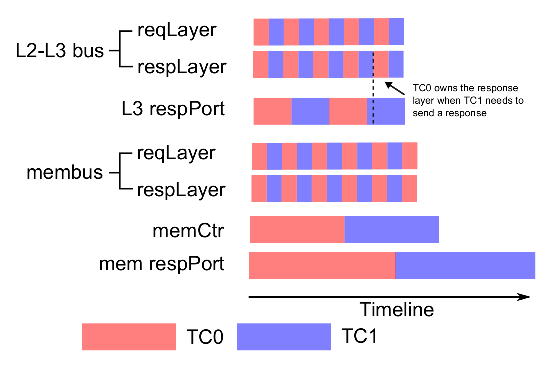
\includegraphics[width=3.46in]{figs/baseline_schedule.eps}
%         \caption{Cache hit timing sequence.}
%         \label{fig:naive_scheme}
%     \end{center}
% \end{figure}
% 
% 
% \begin{figure}
%     \begin{center}
%         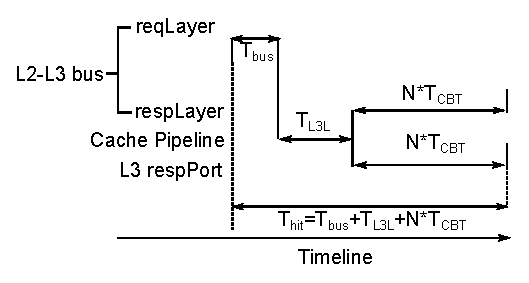
\includegraphics[width=2.4675in]{figs/hit_timing.eps}
%         \caption{L3 cache hit timing sequence.}
%         \label{fig:hit_timing}
%     \end{center}
% \end{figure}
% 
% \begin{figure}
%     \begin{center}
%         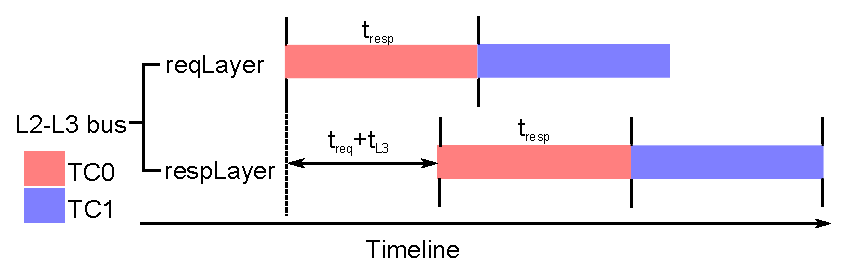
\includegraphics[width=3.2624in]{figs/hit_schedule.eps}
%         \caption{Cache hit timing path schedule.}
%         \label{fig:hit_schedule}
%     \end{center}
% \end{figure}
% 
% \begin{figure}
%     \begin{center}
%         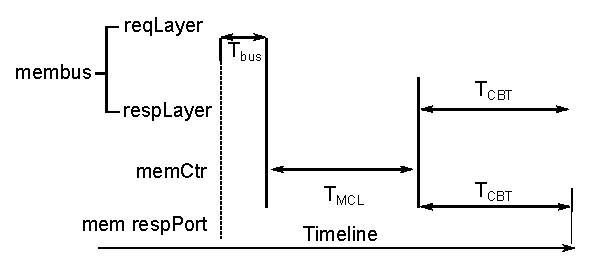
\includegraphics[width=2.9475in]{figs/miss_timing.eps}
%         \caption{The L3-memory timing sequence.}
%         \label{fig:miss_timing}
%     \end{center}
% \end{figure}
% 
% \begin{figure}
%     \begin{center}
%         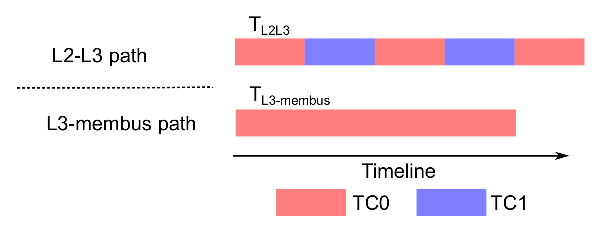
\includegraphics[width=2.9475in]{figs/coordination.eps}
%         \caption{A coordinated cache miss path schedule.}
%         \label{fig:coordination}
%     \end{center}
% \end{figure}

\section{Time Slice Coordination}
\label{sec:coordination}
The Timing Compartments architecture relies heavily on time multiplexing to 
protect shared resources including the L2-L3 bus, the L3-memory bus, and the 
memory controller. These resources frequently interact since each is involved 
in handling L2 misses. If the time multiplexing schedules for each of these 
resources are not designed to account for this interaction, it could lead to 
exorbitant latencies and wasted bandwidth.

\begin{figure}
    \begin{center}
        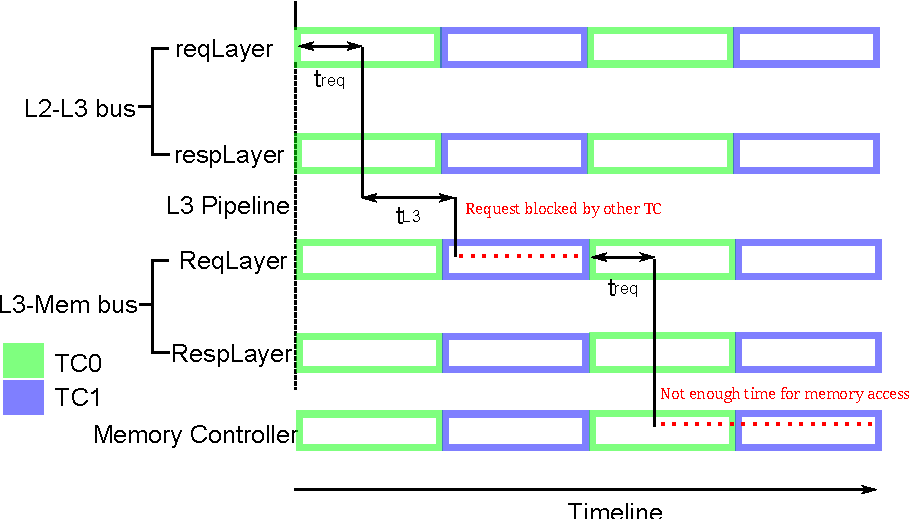
\includegraphics[width=3.5in]{figs/problem.pdf}
        \caption{A poorly performing time multiplexing schedule.}
        \label{fig:problem}
    \end{center}
\end{figure}

Figure \ref{fig:problem}, illustrates the problem. It shows when each of two 
timing compartments are scheduled to use the time multiplexed resources along 
the L2 miss path. Green blocks indicate that TC0 is scheduled to use the device, 
and blue blocks indicate that TC1 is scheduled. We refer to the block of time 
that a timing compartment is scheduled to use a device as the \emph{turn} and 
we refer to the duration of a turn as the \emph{turn length}. In this schedule, 
timing compartments are allotted the same turn length for each time multiplexed 
resource, and the schedule for each device starts at the same time.

%%%%%%%%%%%%%%%%%%%%%%%%%%%%%%%%%%%%%%%%%%%%%%%%%%%%%%%%%%%%%%%%%%%%%%%%%%%%%%%
%% This section is easier to write if we introduce bus layers in the uarch 
%% channel section (section 3)
%%%%%%%%%%%%%%%%%%%%%%%%%%%%%%%%%%%%%%%%%%%%%%%%%%%%%%%%%%%%%%%%%%%%%%%%%%%%%%%
An L3 miss from TC0 is shown proceeding with these time multiplexing schedules.
The miss begins at the L2 request layer where the request is sent to the L3.  
When the L3 access is complete, the request must proceed through the L3-memory 
bus request layer, but at this time TC1 is scheduled to use the L3-memory 
request layer, so it must wait for TC1's turn to finish before the request can 
proceed to the memory controller. Then, when it arrives at the memory 
controller, there is not enough time left in the turn to complete a request, so 
it is blocked again. There are similar issues as the packet traverses the rest
of the path.

Clearly, this schedule is inefficient. When designing a schedule for these 
resources both the L3 hit and L3 miss paths should be considered. In this 
section we describe the timing for both paths. We then show that devising a 
schedule that optimizes just the hit path is straightforward, but scheduling 
the miss path and balancing both is challenging.

\subsection{L2 Miss Timing Paths}
Naturally, to efficiently time multiplex the resources involved in an L2 miss, 
understanding the timing of L2 misses is key. L2 misses take two different 
paths and have different timings depending on whether the L2 miss is an L3 hit 
or miss. Figure \ref{fig:hit_timing} shows the timing for an L3 hit. The arrows 
indicate the time that the resource in the corresponding column is used.

The L2 miss begins by transferring a request over the L2-L3 bus request layer 
in $t_{req}$ cycles. Typically, $t_{req}$ depends on how the bus protocol 
requires requests to be sent. The request then arrives at the L3 cache, where 
it takes $t_{L3}$ cycles (i.e. the L3 cache latency). We assume the cache is 
fully pipelined, so even if a request arrives one cycle after another, both can 
use the cache simultaneously, and the access always completes in $t_{L3}$ 
cycles. Finally, the data is transferred from the L3 response port back to the 
L2 over the L2-L3 bus response layer in $t_{resp}$ cycles. Often, $t_{resp}$ 
will be greater than $t_{req}$. It depends on the bus bandwidth and the size of 
a cache block.

\begin{figure}
    \begin{center}
        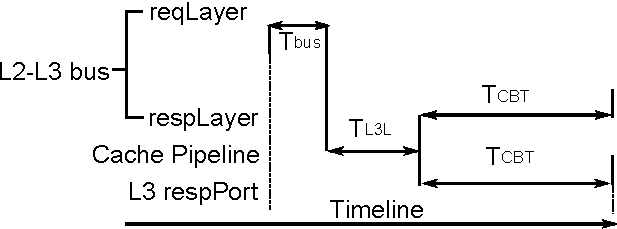
\includegraphics[width=3.5in]{figs/hit_timing.pdf}
        \caption{L3 cache hit timing sequence.}
        \label{fig:hit_timing}
    \end{center}
\end{figure}

Figure \ref{fig:miss_timing} shows the timing for an L3 miss. The request 
begins by transferring over the L2-L3 bus request layer, and similarly takes 
$t_{L3}$ cycles to identify that it is a miss. Afterwards, it sends another 
request to the memory controller over the L3-memory bus request layer in 
$t_{req}$ cycles. Memory requests take variable time to complete, after which 
the data is returned to the L3 in $t_{resp}$ cycles, written to the L3 in 
$t_{L3}$ cycles and finally returned to the L2 after another $t_{resp}$ cycles.

\begin{figure}
    \begin{center}
        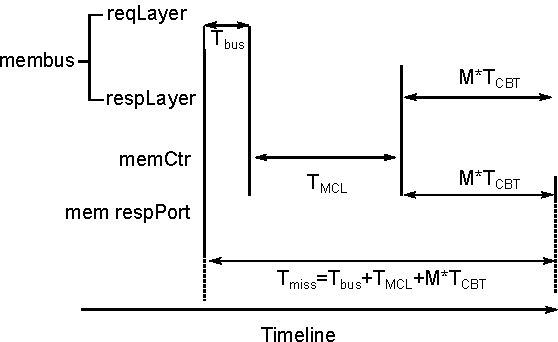
\includegraphics[width=3.5in]{figs/miss_timing.pdf}
        \caption{L3 cache miss timing sequence}
        \label{fig:miss_timing}
    \end{center}
\end{figure}

\subsection{Devising a Schedule}
A good time multiplexing schedule should minimize the L2 miss latency for most 
cases. We can achieve this by controlling the turn lengths and offsets for each 
time multiplexed device. Here, an \emph{offset} refers to a shift in the start 
of the schedule for a single device. Offsets are used to make a resource 
available precisely when the data is available from the preceding resource.

%% A schedule is determined by the set of turn lengths and offsets for each 
%% resource. Turns are allocated for each timing compartment in a repeated 
%% sequence (e.g. 1,2,3,4,1,2,4, for four timing compartments). Therefore, a 
%% schedule for the entire path repeats after the least common multiple of each 
%% turn length in the path multiplied by the number of timing compartments. The 
%% latency for a request can be 

For a particular resource, suitable turn lengths depend on the latency of that 
resource, and suitable offsets depend on the latency of the preceding resource.
This reasoning can be applied in a straightforward way to derive the schedule 
that optimizes the L3 hit path shown in Figure~\ref{fig:hit_schedule}.

The turn length for the L2-L3 request layer must be greater than $t_{req}$. The 
data is available to the L2-L3 response layer after $t_{req}+t_{L3}$ cycles, so 
this is used as the offset for the response layer. The turn length for the 
response layer is $t_{resp}$. Since typically $t_{req}<t_{res}$ we could use a 
shorter turn length for the request layer. However, any requests from one TC 
would be queued until the turn for the same TC on the response layer starts, so 
this provides no benefit. In fact, reducing the turn length causes requests 
that arrive later in the schedule to incur extra delays.

\begin{figure}
    \begin{center}
        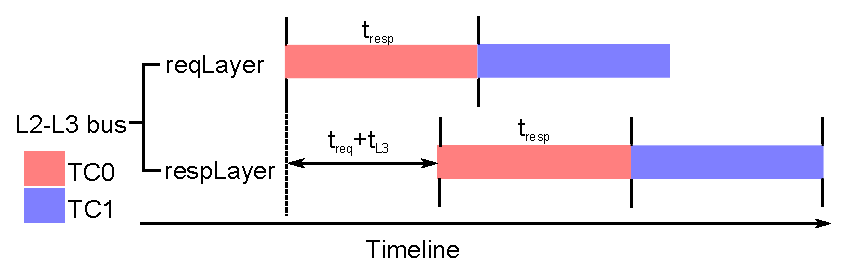
\includegraphics[width=3.2in]{figs/hit_schedule.eps}
        \caption{Cache hit timing path schedule.}
        \label{fig:hit_schedule}
    \end{center}
\end{figure}

Scheduling the L3 miss path is more complicated. The miss path involves two 
more bus layers and the memory controller. The memory accesses take much longer 
than bus transfers and the turn lengths for both can have a large least common 
multiple. As we will show, this can make L2 miss latencies unpredictable if not 
handled well. Further, the memory controller requires a dead time to drain 
in-flight requests and prevent interference. New requests cannot begin during 
the dead time, but old ones can continue. Memory requests must also finish in a 
single turn complicating the schedule even further.

To find the schedule that optimizes the miss path, we used a mix of intuitive
reasoning and integer linear programming optimization techniques, as discussed 
in Section \ref{sec:eval_coord}.
The turn lengths for both L3-memory bus layers and the memory controller are 
$t_{mem}$, the minimum memory turn length. Although these bus turns could have 
been smaller, this would provide no benefit since they transfer responses to 
and from the memory controller exclusively. The L2-L3 bus layer turn lengths 
were the smallest factor of $t_{mem}$ greater than $t_{resp}$. The scaling is 
beneficial since the least common multiple of turn lengths affects the
repeatability of the schedule. The L2-L3 bus turns are increased rather than 
the memory controller since this schedule only optimizes the L3 miss path, not 
the entire L2 miss path. Each device schedule is offset so that it starts when 
the data is available. Table \ref{tab:miss_schedule} summarizes both the turn
lengths and offsets in this schedule. Here $t_{read}$ is the worst case memory
read time, and $t_{resp}^+$ is the smallest factor of $t_{mem}$ greater than 
$t_{resp}$


\begin{table}
    \caption{Optimal L3 Miss Path Schedule}
    \centering
    \begin{tabular}{|r|r|l|l|}
        \hline
        \multicolumn{2}{|l|}{Device Name} & Turn Length & Offset\\\hline
        \multicolumn{2}{|l|}{L2-L3 Req}   & $t_{resp}^+$  & 0\\\hline
        \multicolumn{2}{|l|}{L3-Mem Req}  & $t_{mem}$ & $t_{req}+t_{L3}$\\\hline
        \multicolumn{2}{|l|}{Mem Ctl}     & $t_{mem}$ & $2t_{req}+t_{L3}$\\\hline
        \multicolumn{2}{|l|}{L3-Mem Resp} & $t_{mem}$ & 
          $2t_{req}+t_{L3}+t_{read}$\\\hline
        \multicolumn{2}{|l|}{L2-L3 Resp}  & $t_{resp}^+$ &
          $2t_{req}+2t_{L3}+t_{read}+t_{resp}$\\\hline
    \end{tabular}
    \label{tab:config}
\end{table}



Scheduling the full L2 miss path is even more difficult. Typically getting a 
schedule that repeats in a short period requires increasing either the L3 hit
or miss path. We examined this scheduling problem with linear optimization 
techniques, and although we could not construct much meaning from the optimal 
schedule, we will show in Section \ref{sec:eval_coord} that the gap between
the best and worst schedules is significant. This suggests that although time 
multiplexing the L2 miss path is a difficult problem, it can greatly impact 
performance.
